% GUIDA VELOCE:
% --------------------------------------------------------------------
% X INIZIA UN UNOVO CAPITOLO:
% \chapter{??? NOME CAPITOLO}}
% \section{ ?? }
% \subsection{ ?? }
%
% --------------------------------------------------------------------
% PAROLA CONTENUTA NEL GLOSSARIO:
% scrivere la parola seguita da $^g$
% esempio: User$^g$
%
% --------------------------------------------------------------------
% PER ANDARE A CAPO SENZA RIENTRO INSERIRE:
% \\
%
% --------------------------------------------------------------------
% GRASSETO:
% \textbf{parola}
%
% --------------------------------------------------------------------
% CORSIVO:
% \emph{parola}
% --------------------------------------------------------------------
% PER SCRIVERE IN ROSSO:
% \red{parola}
%
% --------------------------------------------------------------------
% PER SCRIVERE TRA VIRGOLETTE
% ''parola''
%
% --------------------------------------------------------------------
% PER EVITARE IL RIENTRO AUTOMATICO DI UN CAPOVERSO:
% \noindent testo....
%
% --------------------------------------------------------------------

% PER SCRIVERE CARATTERI PARTICOLARI COME: { } _ ecc.. SCRIVERLI PRECEDUTI DA \
% ES: \{ \_
%
% --------------------------------------------------------------------
% X INSERIRE UN LINK:
% \url{http://www.math.unipd.it/~tullio/IS-1/2011/Progetto/C3.pdf}
%
% --------------------------------------------------------------------
% PER COMMENTARE INTERE PARTI:
% \comment{ comment }
%
% --------------------------------------------------------------------
% PER SCRIVERE NOTE DURANTE IL TESTO:
% parola \footnote{ note riguardanti la parola }
%
% --------------------------------------------------------------------
% PER SCRIVERE CODICE SORGENTE:
%
% \lstset{language=c++,
% stringstyle=\color{blue}\textrm,
% commentstyle=\rmfamily, numbers= none}

% \begin{lstlisting}
% CODICE
% \end{lstlisting}
%
% --------------------------------------------------------------------
% !!!!!!!! PER COSE + COMPLESSE VEDI: !!!!!!!!!!!!!!!!!!!!!!!
% !!!!!!!! PMAC/latex/GUIDA LATEX!!!.tex !!!!!!!!!!!!!!!!!!!!!!!

% per tutto il resto chiedi a lory prima di fare/scrivere cazzate !!!!!!!!!!



\documentclass[10pt,a4paper]{book}

\usepackage[italian]{babel}
\usepackage[T1]{fontenc}
\usepackage[utf8x]{inputenc} % uso utf8x xk x linux, mentre latin1 è per windows
\usepackage{lmodern} %insieme di font molto completo consigliato da LatexFacile pg13 in basso
\usepackage{microtype} %migliora riempimento delle righe. vedi LatexImpaziente pg41
%attiva il rientro di ogni prima riga di ogni sezione: capitolo,paragrafo ecc. vd LatexImpaziente pg41
\usepackage{indentfirst}
\usepackage{graphicx} % per inseire immagini
\usepackage[usenames,dvipsnames]{color}
\usepackage{lastpage} %serve per poter scrivere page 1 of N
% setta i bordi della pagina: dx e sx 3.2cm di rientro + nel lato di rilagatura rientra di altri 0mm
\usepackage[a4paper,top=3cm,bottom=3cm,left=3.2cm,right=3.2cm, bindingoffset=0mm]{geometry}
\usepackage{listings} % per inserire codice sorgente
\usepackage{float} % per gestire oggetti flottanti ( es immagini tabelle posizionebili con "H" che forza il posizionamento nel punto specifico )

% serve per creare tabelle lunghe + di una pagina con \begin{longtable} (vd Tabelle.pdf pg11-12)
\usepackage{longtable}

\usepackage{fancyhdr} % per impostare lo stile della pagina più personalizzato, + fancyhdr ( per regolare testatina e piè di pagina ) vedi itfancyhrd

\usepackage{marvosym}


\pagestyle{fancy}
% settaggi di pagestyle(fancy)
\lhead{
\includegraphics[scale=0.20]{images/SevenFold_small}}
%\chead{}
\rhead{\textbf{{%
\NomeDocumento - \VersioneAttuale \\ Data versione attuale: \DataRilascio \\ e-mail: \mail{sevenfold@palomino.it}}}}
\lfoot{\NomeDocumento}
\cfoot{}
\rfoot{ \textbf \thepage\ di \pageref{LastPage}}
\renewcommand{\footrulewidth}{0.4pt}

%ridefinisco il plain per cosare l'indice (a questo punto si potrebbe lasciare tutto il documento in plain
\fancypagestyle{plain}{
\lhead{
\includegraphics[scale=0.20]{images/SevenFold_small}}
%\chead{}
\rhead{\textbf{{%
\NomeDocumento - \VersioneAttuale \\ Data versione attuale: \DataRilascio \\ e-mail: \mail{sevenfold@palomino.it}}}}
\lfoot{\NomeDocumento}
\cfoot{}
\rfoot{ \textbf \thepage\ di \pageref{LastPage}}
\renewcommand{\footrulewidth}{0.4pt}
}

% da ultimo:
\usepackage{hyperref} %x l'interpretazione di indirizzi o link ipertestuali (vd LatexImpaziente pg47 )
\hypersetup{backref, colorlinks=true, linkcolor=black, urlcolor=black}

\usepackage{url} % x l'interpretazioni di internet o link ipertestuali (vd LatexImpaziente pg47 )
%\UrlFont{color =blue}
%\urlstyle{helvetic}

% Define a new 'leo' style for the package that will use a smaller font.
\makeatletter
\def\url@leostyle{%
  \@ifundefined{selectfont}{\def\UrlFont{\sf}}{\def\UrlFont{\small\ttfamily}}}
\makeatother
%% Now actually use the newly defined style.
\urlstyle{leo}


\newcommand{\mail}[1]{\textcolor{Black}{ \texttt{#1}}} %per interpretare mail (vd LatexImpaziente pg47 )
\newcommand{\cambiaFont}[2]{{\fontencoding{T1}\fontfamily{#1}\selectfont#2}}
\newcommand{\red}[1]{ \textcolor{red}{#1} } % per scrivere testo in rosso
\newcommand{\comment}[1]{} % per inserire commenti

\newcommand{\attribute}[2]{ \item[\textcolor{PineGreen}{ \texttt{#1}}] \textcolor{PineGreen}{\texttt{#2\\}}\ \ \ }
\newcommand{\method}[2]{ \item[\textcolor{MidnightBlue}{ \texttt{#1}}] \textcolor{MidnightBlue}{ \texttt{#2\\}}\ \ \ }

\newcommand{ \class}[1]{ \item[-] \texttt{#1} }
\newcommand{\virgolette}[1]{``{#1}''}



% INSERIRE QUI IL NOME DEL DOCUMENTO SEGUITO DA UNO SPAZIO
% ( così il nome si imposta in automatico nelle varie ricorrenze standard)
\newcommand{\NomeDocumento}{Scrivi in questo documento k poi uniamo tutto }

% INSERIRE QUI LA DATA DEL RILASCIO DELLA VERSIONE ATTUALE
\newcommand{\DataRilascio}{2012/04/02}

% INSERIRE LA VERSIONE ATTUALE
\newcommand{\VersioneAttuale}{v2.0.0}

% INSERIRE QUI L'ACRONIMO DEL DOCUMENTO. ESEMPIO: Analisi Dei Requisiti = AR
% Quando inserite l'acronimo qui, dovete rinominare i file presenti nella cartella
% del tipo '??-cap1-NomeCapitolo.tex' sostituendo i '??' con l'acronimo scelto!!
\newcommand{\AcronimoDocumento}{DP}

\begin{document}


% --------------------------------------------------------------------

% TITOLO ( 1° pagina)

\vspace*{2.5cm}
\begin{center}

%\cambiaFont{Cyklop}{Sevenfold}
%\cambiaFont{fve}{\Huge{Sevenfold}}

\includegraphics[scale=0.35]{images/SevenFold_big}

\vspace{2cm}

\cambiaFont{fve}{\Huge{\NomeDocumento}}\\
\vspace*{1cm}

è richiesto: circa 15 pagine a testa..

\end{center}


% --------------------------------------------------------------------

% INFORMAZIONI DEL DOCUMENTO ( 1° pagina)

\vspace*{2cm}




% --------------------------------------------------------------------

% SOMMARIO ( 2° pagina)

\newpage

\vspace*{0.5cm} % il vertical space va preceduto da una riga vuota!!!
\begin{center}

\textbf{{\huge{Sommario}}}

Questo documento contiene la struttura del sistema Woty, analizzando nel dettaglio i suoi componenti.

\vspace*{0.2cm} % il vertical space va preceduto da una riga vuota!!!

\end{center}


% --------------------------------------------------------------------



% --------------------------------------------------------------------
% INDICI:

\newpage

% INDICE CAPITOLI
\tableofcontents % genera l'indice di tutto il documento

\let\cleardoublepage\clearpage % toglie la pagina bianca dopo l'indice

% INDICE TABELLE
\listoftables

% INDICE FIGURE
\listoffigures


% --------------------------------------------------------------------

% INTRODUZIONE ( 1° CAPITOLO ) QUESTO CAPITOLO VA MESSO IN OGNI DOCUMENTO!!!!!!!!

\newpage
\chapter{Business Model}

Il presente descrive il modello di business inteso per la commercializzazione del software Woty. Verranno delineate le caratteristiche di commercializzazione del software, le loro motivazioni e i punti di forza e debolezza.

\section{Ampliamento di Mercato}
Il nostro prodotto inizialmente sarà commercializzato solamente in Italia per approfondire ulteriormente la fattibilità/successo dello stesso e per consolidare la struttura IT su cui si basa e il ramo dell'azienda che segue il progetto.\\
In caso la nostra iniziativa abbia successo e volessimo ampliare il nostro mercato anche in altre regioni
dell'Europa, è da sottolineare che la nostra applicazione supporta già numerose lingue e senza ulteriori fasi
di sviluppo ci si potrebbe dedicare solamente all'ampliamento della struttura IT e della studio dei mercati
europei e delle legislazioni dei singoli paesi in cui si vorrebbe commercializzare il prodotto.

\section{Software as a service}
Come spiegato in precedenza sui dettagli tecnici, il cliente usufruisce dei servizi del software tramite il browser. A differenza dello standard per questo tipo di servizi, Woty necessita di un maggiore grado di rapporto con il cliente a causa della natura eterogenea delle necessità dei clienti. Ogni cliente può avere richieste diverse che almeno inizialmente sono trattate come commesse e sviluppate ad-hoc. In un momento successivo si può pensare alla standardizzazione del servizio e quindi all'apertura verso il mercato mondiale.

%\subsection{Implicazioni commerciali}

%\subsubsection{Acquisizione del cliente}
%Inizialmente vanno gestite commesse per la standardizzazione delle funzionalità. Successivamente il cliente si %arrangia, iscrivendosi e utilizzando autonomamente il servizio.


\section{Business Model}
Andiamo ora a descrivere il business model scelto per affrontare il mercato con il nostro software sia con una descrizione testuale sia con un Canvas che racchiude i concetti chiave.

\subsection{Customer segments}
I customer segment sono i segmenti di mercato al quale il nostro prodotto è rivolto. Il software è stato realizzato tenendo conto delle esigenze specifiche di quelle imprese che hanno bisogno di trovare un'alternativa efficace ai corsi frontali sulla sicurezza, quindi seguiamo un cosiddetto mercato di nicchia, con richieste particolari e raggiungibile tramite canali precisi. \\
Quindi Woty mira a farsi spazio nel mercato attirando clienti che vogliono ridurre le spese per gestire la sicurezza sul lavoro o comunque vogliono affrontare la questione con un approccio innovativo e coinvolgente per i propri dipendenti. \\
Stiamo comunque parlando di un modello B2B, cioè un Business-to-business, che quindi implica che l'acquirente diretto è una società, che poi offrirà il servizio ai suoi dipendenti.\\
\\ \textbf{Concetti chiave:}
\begin{itemize}
\item \textbf{Mercato di nicchia}
\item \textbf{Esigenze specifiche}
\item \textbf{Canali dedicati}
\end{itemize}

\subsection{Value Propositions}
Value Proposition indica il valore proposto al pubblico ed il valore per il quale un customer segment dovrebbe scegliere il nostro prodotto anziché quello di un eventuale concorrente. Questo valore è creato in Woty grazie all'unione di più fattoti chiave che nell'insieme creano un prodotto interessante per la fascia di mercato di destinazione. Vediamoli nello specifico:

\begin{itemize}
\item \textbf{Innovazione}: il software Woty offre un servizio innovativo, che si fa spazio in un settore di mercato ancora poco esplorato. Cerchiamo così di farci notare tra tutti quelli che offrono un servizio simile ma con metodi più tradizionali, perché un mercato non ancora molto sviluppato offre grandi potenzialità di crescita.
\item \textbf{Cost Reduction}: oltre ad innovazione il nostro prodotto offre un metodo per ridurre i costi di formazione del personale, un incentivo non da sottovalutare per utilizzare il nostro prodotto. Sostituendo i corsi frontali sulla sicurezza sul lavoro il nostro software allevia il cliente anche dei costi per sostenere questi corsi, garantendo un margine di risparmio sostanziale. Oltre a pesare sulle finanze del cliente permette un maggiore coinvolgimento da parte dell'utilizzatore finale del prodotto, che spesso può portare ad una formazione del personale migliore.
\item \textbf{Usabilità}: infine il nostro prodotto offre un interfaccia utente facile ed intuitiva per appunto spronare e facilitare l'utilizzo anche da parte di quei clienti meno propensi alle tecnologie informatiche. La parte "social" del nostro prodotto può far ritrovare un ambiente familiare grazie alla grande diffusione dei social network degli ultimi anni.
\end{itemize}

\subsection{Channels}

I canali sono i metodi che abbiamo a disposizione per far arrivare e recepire informazioni e messaggi dalla e verso la clientela, vediamo i channel principali e la loro suddivisione:

\subsubsection{Marketing e pubblicità}

\begin{itemize}
\item \textbf{Inserzioni}\\
Per effettuare un marketing mirato, si è scelto di apportare delle inserzioni pubblicitarie su riviste specialistiche. \\
Tra queste vi è QuotidianoSicurezza.it che consiste in una rivista periodica di aggiornamenti e news sul mondo della sicurezza sul lavoro. In questo modo si può facilmente raggiungere utenti interessati all'ambito della sicurezza sul lavoro e ai metodi innovativi per l'insegnamento della sicurezza sul lavoro in ambito aziendale.\\
QuotidianoSicurezza.it dispone anche di una apposita app per smartphone nella quale vengono visualizzate le news e le inserzioni presenti nel quotidiano.\\
Il preventivo proposto dal quotidiano per la pubblicazione di inserzioni pubblicitarie è di 500\EUR\ ad inserzione. Tale inserzione sarà visibile sia su quotidiano cartaceo che tramite applicazione smartphone.\\ Per il primo anno sono previste tre inserzioni per un costo complessivo di 1500\EUR.\\
\\
La camera di commercio offre la distribuzione gratuita di giornali specifici per ogni categoria commerciale o industriale iscritta al servizio, nei quali sono presenti inserzioni pubblicitarie. La pubblicazione di inserzioni in tali riviste richiede un costo di 350\EUR per inserzione.\\
Per il primo anno sono previste tre inserzioni in tale rivista con un costo complessivo di 1050\EUR.

\item \textbf{Social Network}\\
La promozione di Woty avverrà anche attraverso i principali social network Facebook, Twitter e Google+ con la creazione di una pagina Woty dedicata che ne permetterà una più facile conoscenza.\\
Tutte queste operazioni sono gratuite e non richiedono un esborso di denaro.\\
La pagina per ognuno dei social network dovrà essere mantenuta aggiornata periodicamente per avere maggiore visibilità e interesse nel visitatore.\\
Successivamente, considerato il grande successo del social network Facebook, sarà necessario creare delle inserzioni pubblicitarie in quest'ultimo; le inserzioni permettono di identificare il target di riferimento così da essere mirate per un determinato pubblico di utenza e un tetto massimo di spesa, il cui costo complessivo è previsto per 1200\EUR.

\item \textbf{Affiliazioni}\\
Trattando di sicurezza sul lavoro questo progetto ci offre la possibilità di sfruttare una serie di iniziative di
differenti enti per acquisire visibilità senza spesa alcuna.
Le due maggiori affiliazioni sono:

\begin{itemize}
	\item[\textbf{-}] \textbf{INAIL} (\url{http://www.ispesl.it/scripts/sel_app.asp?area=2&language=1&mod=3}) questo ente offre visibilità gratuita a tutte le iniziative riguardanti il tema di sicurezza degne di nota.

	\item[\textbf{-}] \textbf{EU-OSHA} (\url{http://osha.europa.eu/it}) questo ente offre visibilità gratuita a tutte le iniziative riguardanti il tema di sicurezza degne di nota, inoltre ci permette di fare conoscere la nostra applicazione in ambito europeo offrendoci in futuro la possibilità di introdurre il nostro prodotto in altre nazioni d'Europa.

\end{itemize}

\item \textbf{Rappresentanza}\\
Lavorando in un ambito particolare e delicato che tratta argomenti regolati dalla legge, il nostro progetto richiede una pubblicità mirata che non si riscontra nelle offerte delle agenzie pubblicitarie.\\ Per questo prevediamo la formazione e la mobilitazione di alcuni nostri agenti di commercio. Oltre ad una possibile rappresentanza diretta presso le maggiori aziende del territorio (sfruttando quindi anche il passaparola nell'ambiente aziendale), uno dei principali compiti previsti per queste figure è il contatto degli studi commercialisti del territorio.\\ Questi ultimi, infatti, consigliano la propria clientela in ambito di corsi/sicurezza, indirizzando spesso verso un ente o un servizio privato che offra attestati in materia.\\ Sono da chiarire di persona, ad opera del nostro rappresentante, se sono presenti costi aggiuntivi per far si che gli studi commercialisti pubblicizzino la nostra iniziativa.

\end{itemize}

\subsubsection{Farsi valutare}
\begin{itemize}
\item Il software essendo una web app dispone del sito apposito che ne permette l'utilizzo.\\
Attraverso questo sito vi sarà una apposita sezione per far conoscere Woty agli nuovi utenti indicandone utilizzo, le funzionalità, i piani abbonamento disponibili e molto altro.
\end{itemize}

\subsubsection{Vendità/delivery}
\begin{itemize}
\item Sia l'acquisto che le fornitura del servizio avvengono tramite l'applicazione web, che presenta un form di iscrizione e di scelta del tipo di abbonamento in stile \virgolette{fai da te}, dove il cliente ha tutti i dati per valutare la bontà del servizio e per effettuare la sottoscrizione.
\end{itemize}

\subsubsection{Supporto}
\begin{itemize}
\item Tematico e di post vendita: Il supporto che offriamo al cliente è di tipo self-service od automatico in quanto il cliente ha a disposizione le informazioni per risolvere gli eventuali problemi che riscontra ed in alcuni casi delle procedure guidate. Un esempio è al momento della creazione dell'account dove all'utente viene proposto uno \virgolette{wizard} che lo segue nei primi passi di configurazione. È	 comunque disponibile l'assistenza personale per problemi che non trovano riscontro nelle procedure di risoluzione classiche.
\end{itemize}

\subsection{Customer Relationships}
Descrive il tipo di relazione che la nostra società vuole avere con le fasce di mercato che utilizzano il software Woty. Principalmente cerchiamo di tenere un cosiddetto approccio self-service e di assistenza automatizzata, che quindi implica che l'utilizzatore in caso di bisogno possa trovare tutte le informazioni che gli servono per poter risolvere un eventuale problema. Queste informazioni si possono trovare sia nel manuale di utilizzo software sia negli opportuni "Help" e "About" forniti dall'applicazione Web.\\
Questa scelta è stata fatta per omogenizzare e diminuire il costo del supporto post vendita che data la prevista mole di utilizzatori potrebbe diventare problematica.\\
È comunque previsto il supporto diretto di personale in caso di necessità specifiche o in conseguenza all'acquisto di abbonamenti \textit{Gold}. \\ Tre motivazioni per aver un ottimo rapporto con i clienti.
\begin{itemize}
\item \textbf{Customer Acquisition}: fatta tramite web site e pubblicità.
\item \textbf{Customer Retention}: ottenuta anche con tecniche di gamification (badge e achievement).
\item \textbf{Upselling}: passaparola e reputazione in internet. Un cliente contento parla agli altri del nostro prodotto e consuma mediamente di più.
\end{itemize}
La parte "social" del nostro prodotto aiuta a creare una sorta di community tra gli utilizzatori, fattore che può facilmente portare ad un atteggiamento positivo verso il nostro software, grazie all'ambiente positivo.

\subsection{Revenue Streams}
In base al tipo di prodotto offerto dal software Woty e al suo utilizzo massiccio e sistematico che si avrà all'interno delle aziende acquirenti, si è ritenuto che la licenza abbonamento sia la soluzione più adeguata.\\
La licenza abbonamento prevederà una scadenza annuale rinnovabile, e non saranno richiesti ulteriori costi iniziali di attivazione, in quanto il software prevede una semplice installazione nei pc o smartphone degli utenti utilizzatori di ogni azienda ai quali sarà stato precedentemente assegnato loro un apposito account per effettuare il login alla piattaforma.\\
Per tanto non è necessaria assistenza tecnica specializzata per l'installazione del software.\\
La licenza abbonamento prevederà tre differenti tipologie: \textit{Bronze}, \textit{Silver} e \textit{Gold}.
Di seguito vengono descritte le caratteristiche di ognuna delle licenze sopra elencate:

\begin{itemize}
\item \textbf{\textit{Bronze}}:\\
consiste nella licenza minima.
Può usufruire di tutte le funzionalità base della piattaforma Woty, fatta eccezione dell'applicazione mobile che prevede l'utilizzo del software attraverso smarthphone, pertanto questo tipo di licenza non potrà prevedere account mobile tra gli utenti utilizzatori;


\item \textbf{\textit{Silver}}:\\
La licenza \textit{Silver} prevede tutte le funzionalità della licenza \textit{Bronze}, con l'aggiunta dell'utilizzo dell'applicazione mobile e quindi la possibilità di creare account mobile.
Inoltre è previsto l'uso delle video quest, ossia di quest corredate da un video illustrativo per l'utente;


\item \textbf{\textit{Gold}}:\\
La licenza \textit{Gold} prevede tutte le funzionalità della licenza \textit{Silver}, con l'aggiunta di quest personalizzate per specifici casi o tipi di mansioni in lavori altamente specializzati.\\
Inoltre è prevista un'apposita assistenza tecnica in aggiunta al meccanismo di ticketing già presente nella piattaforma.\\
In caso di problemi urgenti sarà quindi possibile contattare telefonicamente l'assistenza che provvederà a risolvere il problema quanto prima o a fornire istruzioni sul come intervenire.\\

\end{itemize}

Per ognuna delle licenze sopra elencate sarà possibile applicare un numero di licenze di utenti utilizzatori della piattaforma in base al numero di lavoratori presenti nell'azienda acquirente. Tale numero di licenze per utente, potrà essere modificato annualmente allo scadere della licenza annua.\\
Sono previste 5 fasce di numero di utenze che vengono elencate di seguito con i rispettivi costi in base al tipo di licenza scelta:

\begin{table}[ht]

\caption{Licenze previste Woty}
\centering
\begin{tabular}{|p{3cm}|p{1,6cm}|p{1,6cm}|p{1,6cm}|}
\hline
\rule[-2mm]{0mm}{0.7cm}
\textbf{Fascia utenti} &	"\textbf{\textit{Bronze}}" 	& 	"\textbf{\textit{Silver}}" 	& 	"\textbf{\textit{Gold}}"\\
\hline
\rule[-2mm]{0mm}{0.7cm}
"meno di 50"	    &			"500\EUR"	        & 			"750\EUR"			& 			"1.000\EUR"		\\
\hline
\rule[-2mm]{0mm}{0.7cm}
"da 50 a 200"	&			"1.250\EUR"			& 			"1.875\EUR"			& 			"2.500\EUR"		\\
\hline
\rule[-2mm]{0mm}{0.7cm}
"da 200 a 500"	&			"3.500\EUR"			& 			"5.250\EUR"			& 			"7.000\EUR"		\\
\hline
\rule[-2mm]{0mm}{0.7cm}
"da 500 a 1000"	&			"7.500\EUR"			& 			"11.250\EUR"			& 			"15.000\EUR"		\\
\hline
\rule[-2mm]{0mm}{0.7cm}
"più di 1000"	&			"10.000\EUR"			& 			"15.000\EUR"			& 			"20.000\EUR"		\\
\hline
\end{tabular}
\end{table}

\subsection{Key Resources}
Sono le risorse chiave necessarie a fornire e garantire la nostra Value Proposition. Senz'altro in Woty la risorsa che ci permette di offrire il valore che ci contraddistingue è la piattaforma in sé, dato che il suo funzionamento è il principale servizio che offriamo al cliente. Ma le risorse non sono solo fisiche, anche la capacità di offrire nuovi incentivi e soluzioni riguardanti la gamification e i funzionamenti dei "giochi" della piattaforma ideati dal nostro team possono fare la differenza tra un buon prodotto e un prodotto ottimo. Vediamo in dettaglio:
\begin{itemize}
\item \textbf{Risorse fisiche}: struttura fisica che fa funzionare tutto il servizio, deve essere gestita e manutenuta nel migliore dei modi per ridurre le spese ed eventuali incidenti.
\item \textbf{Risorse umane}: team di sviluppo con un know-how tale da organizzare un esperienza di utilizzo e approccio alla gamification che invoglia il cliente all'utilizzo.
\item \textbf{Intellettuali}: miriamo in un periodo di tempo relativamente breve di avere un database di quest e di dati riguardanti la gamification molto amplio, risorsa che può fare la differenza con i nostri competitor.
\end{itemize}

\subsection{Key Activities}
Sono le attività che garantiscono che la nostra Value Proposition possa essere generata, mantenuta e consegnata al cliente. La principale attività che la nostra società deve eseguire è la gestione delle piattaforma che sorregge tutto il software Woty, quindi bisogna controllare sia le risorse fisiche (server) che il software (possibili bug e versioni 2.x).\\
Attività importante è anche la consulenza ai clienti, sia quella personale sia quella automatica (software) che ha bisogno di continue migliorie.\\
Non dimentichiamo che comunque siamo un team di sviluppo software e che quindi un attività fondamentale è quella di aggiornare e migliorare continuamente il nostro codice, sia quello già esistente che quello futuro.

\subsection{Key Partners}
Sono i partner dei quali ci avvaliamo per ottenere vantaggi sia economici che legati all'out\-sourcing. Vediamoli in dettaglio:
\begin{itemize}
\item \textbf{Pubblicità}: la pubblicità sarà in parte affidata e gestita da partner esterni, cosa più economica e conveniente che formare del personale interno.
\item \textbf{Infrastruttura hardware}: la piattaforma hardware sarà fornita e custodita da società terze specializzate in questo tipo di business.	
\item \textbf{Altre alleanze}, sia di tipo strategico che per riduzione dei rischi non sono state programmate per adesso, principalmente per il poco sviluppo del mercato in questo ambito. Non escludiamo partnership con altre società per rafforzare il nostro business in futuro.
\end{itemize}

\subsection{Cost Structure}
È l'insieme delle spese che la nostra attività comporta, sia legate alle infrastrutture che al marketing che alla ricerca e sviluppo. Più è bassa in relazione alle entrate maggiore sarà il reddito della società, quindi si cerca di minimizzare le spese, spinti da un economia di costo più che da una da valore.
\begin{itemize}
\item \textbf{Costi fissi}: i costi fissi previsti per offrire il servizio al cliente sono principalmente quelli legati alla struttura fisica che mantiene attivo il servizio, quelli per il supporto post vendita e gli stipendi di tutti i membri del gruppo.
\item \textbf{Costi variabili}: sono quelli legati alla parte di pubblicità, alle inserzioni e quelli legati alle partnership che eseguono lavori su commissione.
\end{itemize}

Seguiamo un economia di scala in quanto più clienti riusciamo a soddisfare con la nostra infrastruttura e meno ci costerà mantenerla in proporzione ai ricavi. 

\newpage

\subsection{Canvas}

Di seguito viene rappresentato graficamente il riassunto del business model descritto tramite il Canvas dei modelli dei business.

\begin{figure}[H]
\centering
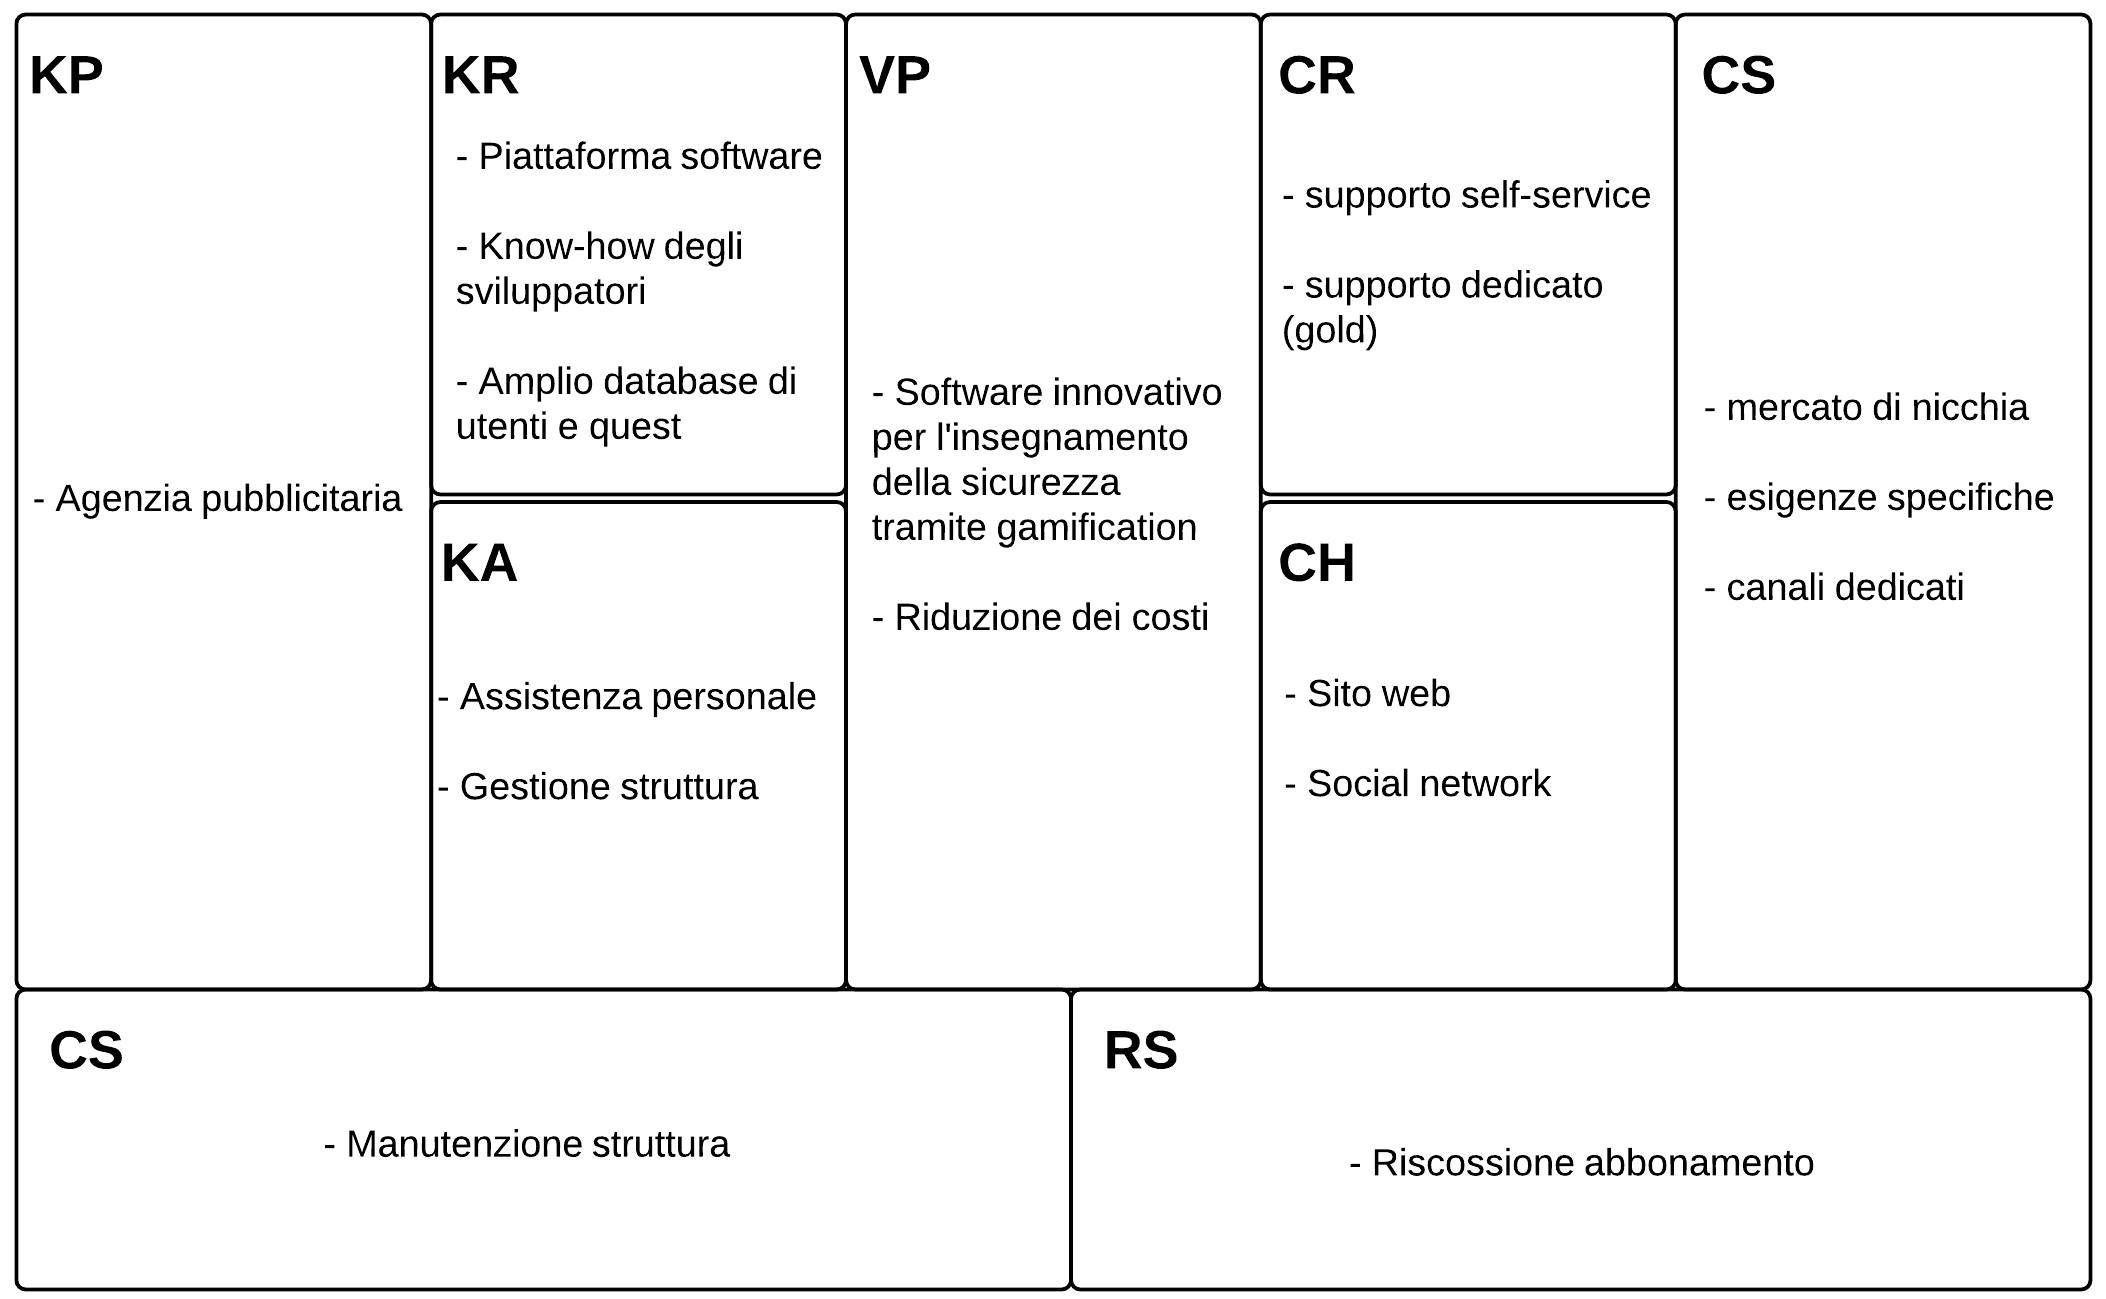
\includegraphics[scale=0.8]{images/BM.png}
\caption{Business Model Canvas}
\end{figure}


\section{Modifiche al software}
A seguito dell'analisi di mercato, dell'analisi sulla concorrenza e dello studio sul business model, si sono riscontrate delle modifiche da effettuare al software in modo da poter essere più competitivo nel mercato e trovare una più facile diffusione presso le aziende.\\
Verrà pertanto riportato in seguito un elenco descrittivo di tali modifiche con l'aggiunta anche delle evenutali estensibilità del sistema, in previsione di modifiche future o adattamenti in fase di manutenzione del software dovuti o a cambiamenti dei requisiti o al riscontro di malfunzionamenti.

\begin{itemize}
\item il sistema già progettato per il supporto al multi lingua, ora dispone solamente delle lingue italiano ed inglese. In seguido allo studio nell'analisi di mercato, si è osservato che i lavoratori stranieri presenti in Italia sono una percentuale non ininfluente. Andranno pertanto aggiunte le traduzioni adeguate per le prinicipali nazionalità dei lavoratori stranienieri;
\underline{tempistiche}: un mese per programmatore e un esperto di lingue;\\
\underline{costo stimato}: 2000\EUR.


\item essendo l'applicazione mobile uno dei punti di forza della piattaforma Woty rispetto ai concorrenti, si prevede la realizzazione dell'applicazione mobile anche per le piattaforme Windows Phone e iOS.
Si potrà così ampliare la gamma dei dispositivi supportati aumentando l'usabilità della piattaforma;\\
\underline{tempistiche}: un mese per due programmatori;\\
\underline{costo stimato}: 4000\EUR.


\item dagli studi sulla concorrenza è emerso come l'uso della gamification per l'insegnamento della sicurezza sul lavoro sia un'innovazione; si prevede quindi di ampliare tale fattore permettendo al sistema la creazione e visualizzazione di nuovi badge;\\
\underline{tempistiche}: una settimana e mezza per un programmatore\\
\underline{costo stimato}: 900\EUR.


\item altro fattore per l'aumento della gamification consiste nell’inserimento di un tempo limite per la risoluzione della quest, l'utente sarà così più motivato nel rispondere correttamente secondo le proprie conoscenze acquisite;\\
\underline{tempistiche}: una settimana per due programmatori\\
\underline{costo stimato}: 600\EUR.

\end{itemize}


Complessivamente gli interventi hanno un costo di circa 7.500 \EUR.




\end{document}